% !TeX document-id = {ac384373-0975-4c4e-b6b2-65611dc82067}
% !TeX TXS-program:compile = txs:///pdflatex/[--shell-escape]
\documentclass[a4paper,12pt]{article}

\usepackage[T2A]{fontenc}
\usepackage[russian]{babel}
\usepackage[intlimits,namelimits]{amsmath}
\usepackage{mathtools}

\usepackage{indentfirst}
\usepackage{icomma}
\usepackage{graphicx}
\usepackage{geometry}
\usepackage{setspace}
\usepackage{fancyhdr}
\usepackage{titlesec}

\usepackage{minted}

\usepackage[bibstyle=gost-numeric,citestyle=numeric-comp]{biblatex}

\usepackage{hyperref}

\addbibresource{biblio.bib}

\geometry{a4paper, nomarginpar, left=20mm, right=10mm, top=20mm, bottom=20mm}

\setlocalecaption{russian}{ref}{Список использованной литературы}

\newcommand\Vect[1]{{\boldsymbol{#1}}}
\newcommand{\dd}{\mathrm{d}}
\newcommand{\diag}{\operatorname{diag}}
\renewcommand{\Re}{\operatorname{Re}}
\renewcommand{\Im}{\operatorname{Im}}
\renewcommand{\exp}{\operatorname{e}}
\renewcommand{\imath}{\mathrm{i}}

\newcommand{\mintedlabel}[1]{\phantomsection\label{\detokenize{#1}}}

% \DeclarePairedDelimeter\bra{\langle}{|}
\DeclarePairedDelimiter\ket{|}{\rangle}
\DeclarePairedDelimiter\abs{\lvert}{\rvert}
\DeclarePairedDelimiterX\commut[2]{[}{]}{#1,#2}

\titlespacing{\section}{\parindent}{3.5ex plus 1ex minus .2ex}{2.3ex plus .2ex}

\fancypagestyle{plain}{%
	\fancyhf{}%
	\fancyfoot[R]{\thepage}%
	\renewcommand{\headrulewidth}{0pt}%
	\renewcommand{\footrulewidth}{0pt}%
}

%%%%%%%%%%%%%%%%%%%%%%%%%%%%%%%%%%%%%%%%%%%%%%%%%%%%%%%%%%%%%%%%%%%%%%%%%%%%%%%%

\makeatletter
\def\@sect[#1]#2{%
	\refstepcounter{app@section}
	\setcounter{equation}{0}
	\addcontentsline{toc}{section}{Приложение~\theapp@section}
	{%
		{
			\raggedleft%
			\normalfont%
			Приложение~\theapp@section\par%
		}%
		\Large\bfseries%
		#2%
		\par%
	}
	\vskip 3ex
}
% This is supposed to be "starred" version, but it doesn't have sense in the
% appendix, so we simply repeat above definition.
\def\@ssect#1{%
	\refstepcounter{app@section}
	\addcontentsline{toc}{section}{Приложение~\theapp@section}%
	{%
		{%
			\raggedleft%
			\normalfont%
			Приложение~\theapp@section\par%
		}%
		\Large\bfseries%
		#1%
		\par%
	}%
	\vskip 3ex
}

\renewcommand\appendix{%
	\newpage%
	\newcounter{app@section}
	\setcounter{app@section}{0}
	%\setcounter{equation}{0}%
	\renewcommand\theapp@section{\Asbuk{app@section}}
	\renewcommand\theequation{\theapp@section\arabic{equation}}
	%%% We need to redefine \section command here...
	%%% NB: this is messy, VERY messy (see GOST for autoreferat!)
	\renewcommand{\section}{%
		\secdef\@sect\@ssect
	}
}

%%%%%%%%%%%%%%%%%%%%%%%%%%%%%%%%%%%%%%%%%%%%%%%%%%%%%%%%%%%%%%%%%%%%%%%%%%%%%%%%

\begin{document}
	\onehalfspacing
	\pagestyle{plain}
	
	\begin{titlepage}
		\begin{center}
			{%
				\scshape
				Министерство высшего образования и науки Российской Федерации\\
			}
			федеральное государственное бюджетное образовательное \\
			учреждение высшего образования \\
			«Иркутский государственный университет»
			(ФГБОУ ВО «ИГУ»)\\
			Физический факультет
		\end{center}
		\vspace*{3em}
		
		\begin{flushright}
			\begin{minipage}{60mm}
				Кафедра теоретической физики\\
				И.о. зав. кафедрой\\
				Доцент, к.ф.-м.н., \underline{\hspace{20mm}} Ловцов С.В.
			\end{minipage}
		\end{flushright}
		\vspace*{4em}
		
		\begin{center}
			\large%
			Курсовая работа\\[2ex]\
			\Large\bfseries%
			Оценка качества численного решения уравнения осцилляций нейтрино в среде
		\end{center}
		
		\vspace*{3em}
		
		\begin{flushright}
			\begin{minipage}{70mm}
				Работы выполнил: \underline{\hspace{30mm}}
				\\[2ex]
				Руководитель: \underline{\hspace{30mm}}\\[2ex]
				Нормоконтроль: \underline{\hspace{30mm}}
			\end{minipage}
		\end{flushright}
		
		\vfill
		\begin{center}
			Иркутск 2024
		\end{center}
	\end{titlepage}
	
	\setcounter{page}{2}
	
	\thispagestyle{empty}
	\tableofcontents
	
	\newpage

	\section{Введение}
	Нейтринная физика сейчас является одним из рубежей современной физики. Также благодаря своим необычным свойствам нейтрино являются важным элементом для построения моделей за пределами стандартной модели.
	
	Нейтрино - это общее название электрически нейтральной фундаментальной частицы
	
	% \newpage
	\section{Уравнение нейтринных осцилляций в среде}
	Когда активные флэйворные нейтрино распространяются в веществе, на их
	эволюционное уравнение влияют эффективные потенциалы из-за когерентного
	взаимодействия со средой посредством реакций нейтрального и заряженного
	токов. Таким образом, влияние среды можно описать в терминах потенциалов, в
	которых распространяются нейтрино, зависящим от состава среды, электрической
	нейтральности, намагниченности (ориентации спинов), скоростей частиц среды.
	
	Когда три известных состояния аромата \(\ket{\nu_{\alpha}}(\alpha= e, \mu, \tau)\) являются линейными комбинациями состояний \(\ket{\nu_{i}}\) c массами \(m_{i}(i=1,2,3)\), состояния флейворных нейтрино являются суперпозицией состояний
	массовых нейтрино
	\begin{equation}\label{eq:1}
		\ket{\nu_{\alpha}}=\sum_{i}U_{\alpha i}^{*}\ket{\nu_{i}},
	\end{equation} 
	Коэффициенты \(U_{\alpha i}\) являются элементами унитарной матрицы
	смешивания \(U\), называемой матрицей Понтекорва–Маки–Накагавы–Сакаты. Для нейтрино Дирака матрица обычно выражается как
	\begin{equation}
		U=O_{23}\Gamma O_{13}\Gamma^{\dagger}O_{12},
	\end{equation}
	где \(O_{ij}\) ортогональные матрицы, представляющие повороты на углы \(\Theta_{ij}\in[0, \pi/2]\) в соответствующих плоскостях, в то время как \(\Gamma=\diag(1,1,\exp^{\imath\delta})\)---диагональная матрица, меняющаяся в пределах \([0, 2\pi]\).
	
	Рассмотрим нейтрино \(\nu_{\alpha}\) рожденное в момент времени
	\(t_{0}\) в среде. Состояние системы \(\ket{\Psi(t)}\) для момента времени \(t\geq t_{0}\) можно представить в виде
	\begin{equation}
		\ket{\Psi(t)}=\sum_{\beta}\Psi_{\beta}(t)\ket{\nu_{\beta}},
	\end{equation}
	Причем \(\Psi_{\beta}(t_{0})=\delta_{\alpha\beta}\). Вероятность иметь состояние аромата \(\beta\) в точке в точке \(r=t (\hbar=c=1)\) равна
	\begin{equation}\label{eq:8}
		P_{\alpha\beta}(r)=|\Psi_{\beta}(r)|^{2}.
	\end{equation}
	После того, как нейтрино покидают среду, амплитуды
	эволюционируют в соответствии с уравнением, которое
	управляет вакуумными колебаниями, решение которого
	проще, если записать его в базисе массовых собственных
	состояний. Используя уравнению \eqref{eq:1}, и обозначив амплитуду вероятности нахождения
	\(\ket{\nu_{j}}\) на краю среды, для \(r\geq r_{*}\) через \(A_{j}=\phi_{j}(r_{*})\), мы получаем
	\begin{equation}\label{eq:7}
		\Psi_{\beta}(r)=\sum_{j=1}^{3}U_{\beta j}A_{j}\exp^{-\imath E_{j}L}
	\end{equation}
	где \(E_{j}=\sqrt{|\Vect{p}|^{2}+m_{j}^{2}}\), \(L=r-r_{*}\) это расстояние
	пройденное нейтрино в вакууме. Теперь в
	уравнении \eqref{eq:8} мы мы используем выражение \eqref{eq:7} и получаем
	\begin{equation}
		P_{\alpha\beta}=\sum_{j}|U_{\beta j}|^{2}|A_{j}|^{2}+2\sum_{i>j}\Re[U_{\beta i}U_{\beta j}^{*}A_{i}A_{j}^{*}\exp^{-\imath\Delta_{ij}L}].
	\end{equation}
	Величина \(\Delta_{ij}=\Delta m_{ij}/2E\), для \(E=|\Vect{p}|\), представляет собой  волновое число колебаний, связанное с квадратом разности масс
	\(\Delta m_{ij}^{2}=m_{i}^{2}-m_{j}^{2}\).
	
	В результате задача вычисления \(P_{\alpha\beta}\) сводится к
	определению величин \(A_{j}\)) т.е. нахождению амплитуд
	собственных массовых состояний \(\phi_{j}(r)\) внутри среды, при начальном условии \(\phi_{j}(r_{0})=U_{\alpha j}^{*}\). Для релятивистских нейтрино, распространяющихся в обычной материи, после вычитания глобальной фазы уравнение эволюции для этих амплитуд имеет вид
	\begin{equation}\label{eq:1}
		\imath\frac{\dd\Phi}{\dd\xi}=[H_{0}+U^{\dagger}VU]\Phi,
	\end{equation}
	где \(\Phi^{T}(r)=(\phi_{1}(\xi),\phi_{2}(\xi),\phi_{3}(\xi))\), \(U\) - матрица
	смешивания, и \(V=\diag(1,0,0)\), \(\xi=\frac{r}{R_{0}}\), где \(R_{0}\) --- солнечный радиус, Первый член в скобках - это матрица Гамильтона, которая управляет эволюцией аромата в вакууме \(H_{0}\), он имеет вид:
	\begin{equation}
		H_{0}=\frac{a}{E}
		\begin{pmatrix}
			0 & 0 & 0\\
			0 & b & 0\\
			0 & 0 & 1
		\end{pmatrix},
	\end{equation}
	
	% \newpage
	\section{Метод численного интегрирования}
	Для численного интегрирования систем дифференциальных уравнений может использоваться семейство методов Рунге-Кутты, метод численного решения задачи Коши для системы обыкновенных дифференциальных уравнений. Самый известный из членов семейства методов Рунге–Кутты часто называется «классическим методом Рунге–Кутты», «RK4» или просто «методом Рунге–Кутты».
	
	начальные условия задачи заданы следующие
	\begin{equation}\label{eq:2} 
		\frac{\dd y}{\dd t}=g(t,y),\qquad y(t_0)=y_0
	\end{equation}
	Здесь, \(y\) — неизвестная функция (скалярная или векторная) времени \(t\),который мы хотели бы приблизить. Утверждается, что \(\frac{\dd y}{\dd t}\) — скорость с которой \(y\) изменяется, является функцией от \(y\) и \(t\). Также \(t_0\), \(y_0\) и функция \(g\) даны.
	
	Необходимо выбрать размер шага \(h>0\), а после определить
	\begin{equation}\label{eq:2} 
		\begin{lgathered}
			y_{n+1}=y_n+\frac{h}{6}(k_1+2k_2+2k_3+k_4),\\
			t_{n+1}=t_n+h,\\
			n=0, 1, 2, 3, 4, ....,\\
		\end{lgathered}
	\end{equation}
	где:    
	\begin{equation}\label{eq:2} 
		\begin{lgathered} 
			k_1=g(t_n, y_n),\\
			k_2=g(t_n+\frac{h}{2}, y_n+h\frac{k_1}{2}),\\
			k_3=g(t_n+\frac{h}{2}, y_n+h\frac{k_2}{2}),\\
			k_3=g(t_n+h, y_n+hl_3),\\
		\end{lgathered}
	\end{equation}
	Здесь \(y_{n+1}\) является RK4 приближением \(y(t_{n+1})\), а следующее значение \(y_{n+1}\) определяется текущим значением \(y_n\) плюс средневзвешенное значение четырех приращений, где каждое приращение является произведением размера интервала \(h\) и предполагаемого наклона, заданного функцией \(g\) в правой части дифференциального уравнения (рис.\ref{fig:magnus}).
	\begin{figure}[htb]
		\centering%
		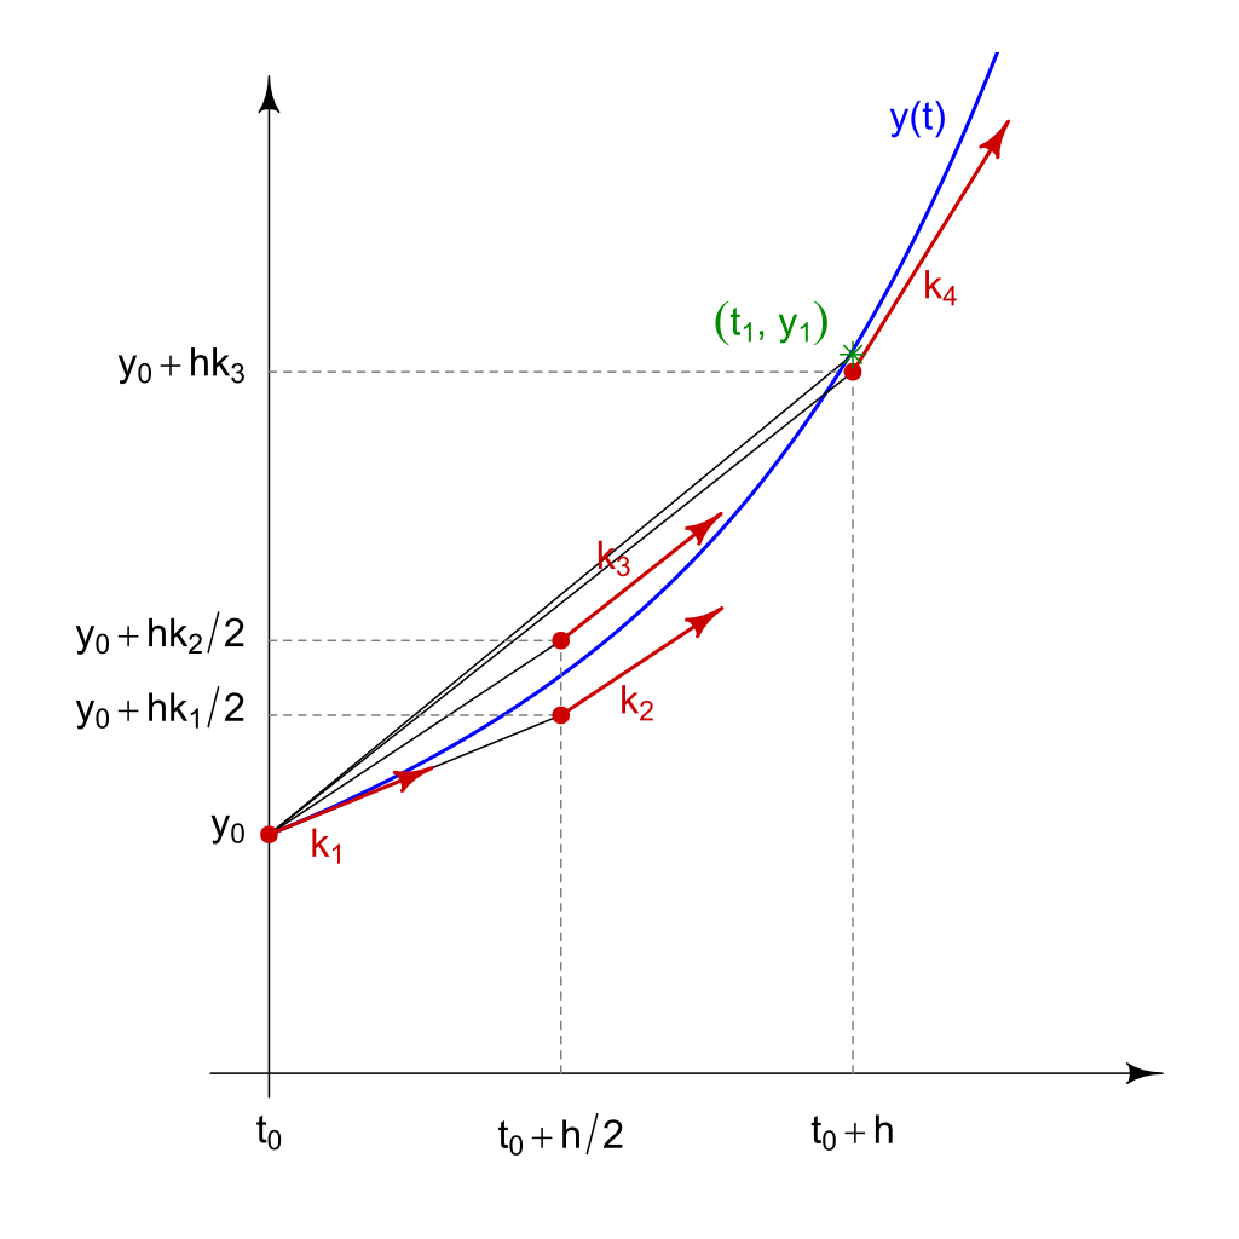
\includegraphics[width=0.8\linewidth]{Ruhgy_koef}
		\caption{\label{fig:magnus}Уклоны, используемые классическим методом Рунге-Кутта}
	\end{figure}
	
	Метод RK4 является методом четвертого порядка, что означает, что локальная ошибка усечения имеет порядок \(O(h^{5})\), в то время как общая накопленная ошибка составляет порядка\(O(h^{4})\).
	
	Семейства методов Рунге-Кутты бывают явными и неявными. В явных методах Рунге-Кутты значения вычисляются только по предыдущим значениям, а в неявных методах Рунге-Кутты значения вычисляются как и по предыдущим, так и по последующим значениям. Семейство явных методов Рунге–Кутты задается формулой
	\begin{equation}\label{eq:2} 
		y_{n+1}=y_n+h\sum_{i=1}^{s}b_ik_i,
	\end{equation}
	где
	\begin{equation}\label{eq:2} 
		\begin{lgathered} 
			k_1=g(t_n, y_n),\\
			k_2=g(t_n+c_2h, y_n+a_{21}k_1h),\\
			k_3=g(t_n+c_3h, y_n+(a_{31}k_1+a_{32}k_1)),\\
			\vdots\\
			k_s=g(t_n+c_sh, y_n+h\sum_{i=1}^{s-1}a_{si}k_i),\\
		\end{lgathered}
	\end{equation}
	
	Чтобы указать конкретный метод, необходимо указать целое число \(s\) (количество стадий) и коэффициенты \(a_{ij}\) (для 1 \(\leq\) j < i \(\leq\) s ), \(b_i\) (для i = 1, 2, ..., s ) и \(c_i\) (для i = 2, 3, ..., s ). Матрица \([a_{ij}]\) называется матрицей Рунге–Кутты , тогда как \(b_i\) и \(c_i\) известны как веса и узлы . Эти данные обычно предоставляются в виде таблицы Бутчера.
	\[
	\renewcommand\arraystretch{1.2}
	\begin{array}
		{c|ccccc}
		0\\
		c_2 &a_{21}\\
		c_3 &a_{31} &a_{32}\\
		\vdots &\vdots & &\ddots\\
		c_s& a_{s1} &a_{s2}& \ldots&a_{s,s-11}\\
		\hline
		& b_1 &b_2 &\ldots &b_{s-1} &b_s
	\end{array}
	\]
	Разложение в ряд Тейлора показывает , что метод Рунге–Кутты является последовательным тогда и только тогда, когда
	\begin{equation}\label{eq:2} 
		\sum_{i=1}^{s}b_i=1.
	\end{equation}
	 если явный \(s\)-этапный метод Рунге–Кутты имеет порядок \(p\), что означает, что локальная ошибка усечения равна \(O(h^{p+1})\), то можно доказать, что число стадий должно удовлетворять \(s\geq p\), а если \(p\geq 5\) то \(s\geq p+1\). Однако неизвестно, являются ли эти границы точными во всех случаях. В некоторых случаях доказано, что граница не может быть достигнута. Например, Бутчер доказал, что для \(p>6\), нет явного метода с \(s=p+1\). Бутчер также доказал, что для \(p>7\) не существует явного метода Рунге-Кутты с \(p+2\). Однако, в целом, остается открытым вопрос о том, какое точное минимальное число стадий \(p\).
	 
	 Метод RK4 попадает в эту структуру. Его таблица
	 \[
	 \renewcommand\arraystretch{1.2}
	 \begin{array}
	 	{c|cccc}
	 	0\\
	 	\frac{1}{2} & \frac{1}{2}\\
	 	\frac{1}{2} &0 &\frac{1}{2} \\
	 	1& 0& 0& 1\\
	 	\hline
	 	& \frac{1}{6} &\frac{1}{3} &\frac{1}{3} &\frac{1}{6} 
	 \end{array}
	 \]
\end{document}

